
% \section{BÀI TẬP ÔN TẬP CHƯƠNG I}
\Opensolutionfile{ans}[ans/ans-1K1-4-OTC]
\begin{ex}%[Câu 1]%[1K1Y1-1]
	Đổi $225^\circ$ sang rađian.
	\choice
	{$\dfrac{4\pi}{5}$}
	{$\dfrac{6\pi}{5}$}
	{$\dfrac{3\pi}{7}$}
	{\True $\dfrac{5\pi}{4}$}
	%<MyLT2>
	\loigiai{
		Ta có $225^\circ = \dfrac{225}{180}\pi=\dfrac{5\pi}{4}$ (rađian).
	}
\end{ex}
\begin{ex}%[Câu 2]%[1K1Y1-3]
	Một đường tròn có bán kính $R=10$ cm. Độ dài cung $40^\circ$ trên đường tròn gần bằng
	\choice
	{$11$ cm}
	{$13$ cm}
	{\True $7$ cm}
	{$9$ cm}
	\loigiai{
		Ta có $40^\circ = 40\cdot \dfrac{\pi}{180} =\dfrac{2\pi}{9}$ rađian.\\
		Độ dài cung $l=\dfrac{2\pi}{9}\cdot 10=\dfrac{20\pi}{9}\approx 7$ cm.
	}
\end{ex}
\begin{ex}%[Câu 3]%[1K1B1-4]
	Bánh xe của người đi xe đạp quay được $2$ vòng trong $6$ giây. Hỏi trong $1$ giây, bánh xe quay được bao nhiêu độ?
	\choice
	{$60^\circ$}
	{$72^\circ$}
	{$240^\circ$}
	{\True $120^\circ$}
	\loigiai{
		Trong $6$ giây, bánh xe quay được $2\cdot 360^\circ=720^\circ$.\\
		Trong $1$ giây, bánh xe quay được $720^\circ\colon 6=120^\circ$.
	}
\end{ex}
\begin{ex}%[Câu 4]%[1K1Y1-6]
	Cho góc $\alpha$ thỏa mãn $90^\circ <\alpha <180^\circ$. Khẳng định nào sau đây đúng?
	\choice
	{$\cos\alpha>0$}
	{\True $\sin\alpha>0$}
	{$\tan\alpha>0$}
	{$\cot\alpha>0$}
	\loigiai
	{Vì $90^\circ <\alpha <180^\circ$ nên $\sin\alpha>0$, $\cos\alpha<0$, $\tan\alpha<0$ và $\cot\alpha<0$.}
\end{ex}
\begin{ex}%[Câu 5]%[1K1B1-6]
	Cho $\sin \alpha =\dfrac{1}{3}$ và $\dfrac{\pi}{2}<\alpha<\pi$. Khi đó $\cos \alpha$ có giá trị là
	\choice
	{$\cos \alpha =-\dfrac{2}{3}$}
	{$\cos \alpha =\dfrac{2\sqrt{2}}{3}$}
	{$\cos \alpha =\dfrac{8}{9}$}
	{\True $\cos \alpha =-\dfrac{2\sqrt{2}}{3}$}
	\loigiai{
		Ta có $\cos^2 \alpha =1-\sin^2 \alpha =1-\left(\dfrac{1}{3}\right)^2=\dfrac{8}{9}$.\\
		Vì $\dfrac{\pi}{2}<\alpha<\pi$ nên $\cos \alpha <0$.\\
		Do đó $\cos \alpha =-\dfrac{2\sqrt{2}}{3}$.
	}
\end{ex}
\begin{ex}%[Câu 6]%[1K1B1-7]
	Cho $A$, $B$, $C$ là ba góc của tam giác $ABC$. Trong các khẳng định sau, khẳng định nào \textbf{sai}?
	\choice
	{$\sin (B+C)=\sin A$}
	{$\cos (B+C)=-\cos A$}
	{\True $\tan (B+C)=\tan A$}
	{$\cot (B+C)=-\cot A$}
	\loigiai{
		Ta có $B+C=180^\circ-A$.\\Suy ra $\tan(B+C)=\tan (180^\circ-A)=-\tan A$.
	}
\end{ex}
\begin{ex}%[Câu 7]%[1K1B1-8]
	Tính giá trị biểu thức $P=\cos ^2\dfrac{\pi}{8}+\cos ^2\dfrac{{3\pi}}{8}+\cos ^2\dfrac{{5\pi}}{8}+\cos ^2\dfrac{{7\pi}}{8}.$
	\choice
	{$P=-1$}
	{$P=0$}
	{$P=1$}
	{\True $P=2$}
	\loigiai{Ta có $\cos ^2\dfrac{7\pi}{8}=\cos ^2\dfrac{\pi}{8}$ và $\cos ^2\dfrac{5\pi}{8}=\cos ^2\dfrac{3\pi}{8}$
		$\Rightarrow P=2\left({{\cos}^2\dfrac{\pi}{8}+{\cos}^2\dfrac{{3\pi}}{8}}\right)$.\\
		Vì $\dfrac{\pi}{8}+\dfrac{{3\pi}}{8}=\dfrac{\pi}{2}\Rightarrow \cos \dfrac{\pi}{8}=\sin \dfrac{{3\pi}}{8}\Rightarrow \cos ^2\dfrac{\pi}{8}=\sin ^2\dfrac{{3\pi}}{8}.$\\
		Do đó $ P=2 \left({{\sin}^2\dfrac{{3\pi}}{8}+{\cos}^2\dfrac{{3\pi}}{8}}\right)=2\cdot1=2.$
	}
\end{ex}
\begin{ex}%[Câu 8]%[1K1B1-8]
	Cho $\sin a + \cos a = - \dfrac 54$, khi đó giá trị của $\sin a \cos a$ bằng
	\choice
	{$1$}
	{$\dfrac{5}{4}$}
	{$\dfrac{3}{16}$}
	{\True $\dfrac{9}{32}$}
	\loigiai{
		$\sin a\cos a = \dfrac{(\sin a + \cos a)^2 -1}{2} = \dfrac{9}{32}$.
	}
\end{ex}
\begin{ex}%[Câu 9]%[1K1Y1-8]
	Cho $\tan x=\dfrac{1}{2}$. Tính $\tan \left(x+\dfrac{\pi}{4}\right)$.
	\choice
	{$2$}
	{$\dfrac{3}{2}$}
	{$6$}
	{\True $3$}
	\loigiai
	{
		Ta có $\tan \left(x+\dfrac{\pi}{4}\right)=\dfrac{\tan x+\tan \dfrac{\pi}{4}}{1-\tan x\cdot \tan \dfrac{\pi}{4}}=\dfrac{\dfrac{1}{2}+1}{1-\dfrac{1}{2}} = 3$.
	}
\end{ex}
\begin{ex}%[Câu 10]%[1K1Y1-3]
	Biểu diễn các góc lượng giác $\alpha=-\dfrac{5\pi}{6}$, $\beta=\dfrac{\pi}{3}$, $\gamma=\dfrac{25\pi}{3}$, $\delta=\dfrac{17\pi}{6}$ trên đường tròn lượng giác. Các góc nào có điểm biểu diễn trùng nhau?
	\choice
	{\True $\beta$ và $\gamma$}
	{$\alpha$, $\beta$, $\gamma$}
	{$\beta$, $\gamma$, $\delta$}
	{$\alpha$ và $\beta$}
	\loigiai{
		Ta có $\beta+8\pi=\dfrac{\pi}{3}+8\pi=\dfrac{25\pi}{3}=\gamma$.\\
		Do đó, $\beta$ và $\gamma$ có điểm biểu diễn trùng nhau trên đường tròn lượng giác.
	}
\end{ex}
\begin{ex}%[Câu 11]%[1K1Y1-7]
	Trong các khẳng định sau, khẳng định  nào là \textbf{sai}?
	\choice
	{$\sin(\pi-\alpha)=\sin\alpha$}
	{\True $\cos(\pi-\alpha)=\cos \alpha$}
	{$\sin(\pi+\alpha)=-\sin\alpha$}
	{$\cos(\pi+\alpha)=-\cos \alpha$}
	\loigiai{
		Ta có $\cos(\pi-\alpha)=-\cos \alpha$ nên $\cos(\pi-\alpha)=\cos \alpha$ là khẳng định \textbf{sai}.
	}
\end{ex}
\begin{ex}%[Câu 12]%[1K1Y1-2]
	Góc lượng giác nào tương ứng với chuyển động quay $3\dfrac{1}{5}$ vòng ngược chiều kim đồng hồ?
	\choice
	{$\dfrac{16 \pi}{5}$}
	{$\left(\dfrac{16}{5}\right)^\circ$}
	{\True $1152^\circ$}
	{$1152 \pi$}
	\loigiai{
		Chuyển động quay ngược chiều kim đồng hồ là quay theo chiều dương; góc tương ứng là
		$$3\dfrac{1}{5}\cdot 2\pi=\dfrac{32\pi}{5}, \text{ tương ứng với } 1152^\circ.$$
	}
\end{ex}

\begin{ex}%[Câu 13]%[1K1Y2-1]
	Trong các khẳng định sau, khẳng định nào \textbf{sai}?
	\choice
	{\True $\cos (a-b)=\cos a\cos b-\sin a\sin b$}
	{$\sin (a-b)=\sin a\cos b-\cos a\sin b$}
	{$\cos (a+b)=\cos a\cos b-\sin a\sin b$}
	{$\sin (a+b)=\sin a\cos b+\cos a\sin b$}
	\loigiai{
		Ta có $\cos (a-b)=\cos a\cos b+\sin a\sin b$ nên $\cos (a-b)=\cos a\cos b-\sin a\sin b$ là khẳng định \textbf{sai}.
	}
\end{ex}
\begin{ex}%[Câu 14]%[1K1Y1-7]
	Trong trường hợp nào dưới đây $\cos \alpha=\cos \beta$ và $\sin \alpha=-\sin \beta$?
	\choice
	{\True $\beta=-\alpha$}
	{$\beta=\pi-\alpha$}
	{$\beta=\pi+\alpha$}
	{$\beta=\dfrac{\pi}{2}+\alpha$}
	\loigiai{
		Trong trường hợp hai cung đối nhau thì các giá trị $\cos$ của chúng bằng nhau, các giá trị $\sin$ của chúng đối nhau.
	}
\end{ex}

\begin{ex}%[Câu 15]%[1K1B2-2]
	Nếu $\cos a=\dfrac{1}{4}$ thì $\cos 2 a$ bằng
	\choice
	{$\dfrac{7}{8}$}
	{\True $-\dfrac{7}{8}$}
	{$\dfrac{15}{16}$}
	{$-\dfrac{15}{16}$}
	\loigiai{
		Ta có  $\cos 2 a =2 \cos^2 a-1=2 \cdot \left( \dfrac{1}{4} \right)^2-1=-\dfrac{7}{8}$.
	}
\end{ex}
\begin{ex}%[Câu 16]%[1K1K2-2]
	Nếu $\tan (a+b)=3, \tan (a-b)=-3$ thì $\tan 2 a$ bằng
	\choice
	{\True $0$}
	{$\dfrac{3}{5}$}
	{$1$}
	{$-\dfrac{3}{4}$}
	\loigiai{
		Ta có $\tan (a+b)=3 \Leftrightarrow \tan a+ \tan b= 3- 3 \tan a \tan b$ \quad (1)\\
		và 
		$\tan (a-b)=-3 \Leftrightarrow \tan a- \tan b= -3- 3 \tan a \tan b$. \quad (2) \\
		Lấy vế trừ vế của (1) và (2) ta được $2\tan b=6\Leftrightarrow \tan b =3$.\\
		Thay $\tan b =3$ vào (1) ta được $\tan a= 0$.\\
		Khi đó $\tan 2 a = \dfrac{2 \tan a}{1- \tan^2 a}=0$.
	}
\end{ex}

\begin{ex}%[Câu 17]%[1K1K2-3]
	Nếu $\cos a=\dfrac{3}{5}$ và $\cos b=-\dfrac{4}{5}$ thì $\cos (a+b) \cos (a-b)$ bằng
	\choice
	{\True $0$}
	{$2$}
	{$4$}
	{$5$}
	\loigiai{
		Do  $\cos a=\dfrac{3}{5}$ và $\cos b=-\dfrac{4}{5}$ nên  $\cos 2a=-\dfrac{7}{25}$ và $\cos 2b=\dfrac{7}{25}$.\\
		Ta có $2 \cos (a+b) \cos (a-b)= \cos 2a +\cos 2b=-\dfrac{7}{25}+ \dfrac{7}{25}=0$.\\
		Do đó $\cos (a+b) \cos (a-b)=0$.
	}
\end{ex}




\begin{ex}%[Câu 18]%[1K1B2-3]
	Rút gọn biểu thức $M=\cos(a+b)\cos(a-b)-\sin (a+b)\sin(a-b)$, ta được
	\choice
	{$M=\sin 4a$}
	{$M=1-2\cos^2a$}
	{\True $M=1-2\sin^2a$}
	{$M=\cos 4a$}
	\loigiai{
		Ta có
		\allowdisplaybreaks
		\begin{eqnarray*}
			M&=&\cos(a+b)\cos(a-b)-\sin (a+b)\sin(a-b)\\
			&=&\dfrac{1}{2}\left(\cos2a+\cos 2b\right)+\dfrac{1}{2}\left(\cos2a-\cos 2b\right)\\
			&=&\cos 2a\\
			&=&1-2\sin^2a.
		\end{eqnarray*}
	}
\end{ex}
\begin{ex}%[Câu 19]%[1K1B2-2]
	Nếu $\sin x +\cos x = \dfrac{1}{2}$ thì $\sin 2x$ bằng
	\choice
	{$\dfrac{3}{4}$}
	{$\dfrac{3}{8}$}
	{$\dfrac{\sqrt{2}}{2}$}
	{\True $-\dfrac{3}{4}$}
	\loigiai{
		Ta có $\sin 2x=\left( {\sin x+\cos x} \right)^2-\left( {\sin^2 x+\cos ^2x} \right)=\left( {\dfrac{1}{2}} \right)^2-1=-\dfrac{3}{4}$.}
\end{ex}
\begin{ex}%[Câu 20]%[1K1Y2-3]
	Mệnh đề nào dưới đây đúng?
	\choice
	{\True $\cos3x\cdot\cos5x=\dfrac{1}{2}(\cos8x+\cos2x)$}
	{$\cos3x\cdot\cos5x=\dfrac{1}{2}(\cos8x-\cos2x)$}
	{$\cos3x\cdot\cos5x=\dfrac{1}{2}(\cos2x-\cos8x)$}
	{$\cos3x\cdot\cos5x=\dfrac{1}{2}(\sin8x+\sin2x)$}
	\loigiai{Ta có $\cos3x\cdot\cos5x=\dfrac{1}{2}[\cos(3x+5x)+\cos(3x-5x)]=\dfrac{1}{2}(\cos8x+\cos2x)$.}
\end{ex}
\begin{ex}%[Câu 21]%[1K1B2-4]
	Giả sử $3\sin ^4x-\cos ^4x=\dfrac{1}{2}$ thì $\sin ^4x+3\cos ^4x$ có giá trị bằng
	\choice
	{$2$}
	{\True $1$}
	{$4$}
	{$3$}
	\loigiai{
		\begin{eqnarray*}
			3\sin ^4x-\cos ^4x=\dfrac{1}{2}\Leftrightarrow 6\sin ^4x-2\cos ^4x=1&\Leftrightarrow& 6\sin ^4x-2\left(1-\sin^2\alpha\right)^2=1\\
			&\Leftrightarrow& 4\sin ^4x-4\sin ^2\alpha-3=0\\
			&\Leftrightarrow& \left(2\sin^2\alpha+3\right)\left(2\sin^2\alpha-1\right)=0\\
			&\Rightarrow&{\sin ^2}\alpha=\dfrac{1}{2}.
		\end{eqnarray*}
		Ta có $\sin ^4x+3\cos ^4x$ $=\sin ^4\alpha+3\left(1-\sin^2\alpha\right)^2$ $=\dfrac{1}{4}+3\left(1-\dfrac{1}{2}\right)^2=1$.}
\end{ex}
\begin{ex}%[Câu 22]%[1K1B3-2]
	Hàm số $y=\sin x$ đồng biến trên khoảng
	\choice
	{$(0 ; \pi)$}
	{$\left(-\dfrac{3 \pi}{2} ;-\dfrac{\pi}{2}\right)$}
	{\True $\left(-\dfrac{ \pi}{2} ;\dfrac{\pi}{2}\right)$}
	{$(-\pi ; 0)$}
	\loigiai{ 
		Do hàm số $y=\sin x$ đồng biến trên mỗi khoảng $\left( -\dfrac{\pi}{2}+k2 \pi;\dfrac{\pi}{2}+k2 \pi \right) $ nên ứng với $k=0$, ta có hàm số $y=\sin x$ đồng biến trên khoảng $\left(-\dfrac{ \pi}{2} ;\dfrac{\pi}{2}\right)$.
	}
\end{ex}

\begin{ex}%[Câu 23]%[1K1B3-2]
	Hàm số nghịch biến trên khoảng $(\pi ; 2 \pi)$ là
	\choice
	{$y=\sin x$}
	{$y=\cos x$}
	{$y=\tan x$}
	{\True $y=\cot x$}
	\loigiai{
		Do hàm số $y=\cot x$ nghịch biến trên mỗi khoảng $\left( k \pi; \pi +k \pi \right) $ nên  ứng với $k=1$, ta có hàm số $y=\cot x$ nghịch biến trên khoảng $(\pi ; 2 \pi)$.
	}
\end{ex}
\begin{ex}%[Câu 24]%[1K1B3-1]
	Tập xác định của hàm số $y=\dfrac{\cos x}{\sin x-1}$ là
	\choice
	{$\mathbb{R}\setminus \left\{k2\pi| k\in\mathbb{Z}\right\}$}
	{\True $\mathbb{R}\setminus \left\{\dfrac{\pi}{2}+k2\pi| k\in\mathbb{Z}\right\}$}
	{$\mathbb{R}\setminus \left\{\dfrac{\pi}{2}+k\pi| k\in\mathbb{Z}\right\}$}
	{$\mathbb{R}\setminus \left\{k\pi| k\in\mathbb{Z}\right\}$}
	\loigiai{
		Hàm số xác định khi và chỉ khi $\sin x-1\ne 0\Leftrightarrow\sin x\ne 1\Leftrightarrow x\ne \dfrac{\pi}{2}+k2\pi$ với $k\in \mathbb{Z}$.\\
		Vậy tập xác định của hàm số là $\mathbb{R}\setminus \left\{\dfrac{\pi}{2}+k2\pi| k\in\mathbb{Z}\right\}$.
	}
\end{ex}
\begin{ex}%[Câu 25]%[1K1Y3-1]
	Khẳng định nào sau đây là \textbf{sai}?
	\choice
	{Hàm số $y=\cos x$ có tập xác định là $\mathbb{R}$}
	{Hàm số $y=\cos x$ có tập giá trị là $[-1;1]$}
	{\True Hàm số $y=\cos x$ là hàm số lẻ}
	{Hàm số $y=\cos x$ tuần hoàn với chu kì $2\pi$}
	\loigiai{
		Hàm số $y=\cos x$ là hàm số chẵn.
	}
\end{ex}
\begin{ex}%[Câu 26]%[1K1Y3-4]
	Trong các hàm số sau đây, hàm số nào là hàm tuần hoàn?
	\choice
	{$y=\tan x+x$}
	{$y=x^2+1$}
	{\True $y=\cot x$}
	{$y=\dfrac{\sin x}{x}$}
	\loigiai{
		Hàm số $y=\cot x$ là hàm số tuần hoàn với chu kỳ $T=\pi$.
	}
\end{ex}
\begin{ex}%[Câu 27]%[1K1Y3-3]
	Khẳng định nào sau đây đúng?
	\choice
	{Hàm số $y=\sin x$ là hàm số chẵn}
	{\True Hàm số $y=\cos x$ là hàm số chẵn}
	{Hàm số $y=\tan x$ là hàm số chẵn}
	{Hàm số $y=\cot x$ là hàm số chẵn}
	\loigiai{
		Hàm số $y=\cos x$ là hàm số chẵn;  các hàm số còn lại là hàm số lẻ.
	}
\end{ex}
\begin{ex}%[Câu 28]%[1K1B3-3]
	Khẳng định nào sau đây là đúng?
	\choice
	{Hàm số $y=\cos x$ là hàm số lẻ}
	{\True Hàm số $y=\tan 2x- \sin x$ là hàm số lẻ}
	{Hàm số $y=\sin x$ là hàm số chẵn}
	{Hàm số $y=\tan x \cdot \sin x$ là hàm số lẻ}
	\loigiai{
		Xét hàm số $y=f\left( {x} \right)=\tan 2x-\sin x$.
		\\Hàm số xác định khi $\cos 2x \ne 0 \Leftrightarrow x \ne \dfrac{\pi}{4}+k\dfrac{\pi}{2}$, $\left( {k \in \mathbb{Z}} \right)$.
		\\Tập xác định $\mathscr{D}=\mathbb{R} \setminus \left\{ {\dfrac{\pi}{4}+k\dfrac{\pi}{2},k \in \mathbb{Z}} \right\}$.
		\\ Với mọi $x \in \mathscr{D}$ thì $-x \in \mathscr{D}$ và $f\left( {-x} \right)=\tan \left( {-2x} \right)- \sin \left( {-x} \right)=-\tan 2x + \sin x=-f\left( {x} \right)$.\\ Do đó hàm số $y=\tan 2x-\sin x$ là hàm số lẻ.}
\end{ex}
\begin{ex}%[Câu 29]%[1K1B3-1]
	Tập xác định của hàm số $y=\dfrac{\cot x}{\cos x-1}$ là
	\choice
	{$\mathbb{R}\setminus\left\{\dfrac{k\pi}{2}, k\in\mathbb{Z}\right\}$}
	{$\mathbb{R}\setminus\left\{\dfrac{k}{2}+k\pi, k\in\mathbb{Z}\right\}$}
	{\True $\mathbb{R}\setminus\left\{k\pi, k\in\mathbb{Z}\right\}$}
	{$\mathbb{R}\setminus\left\{k2\pi, k\in\mathbb{Z}\right\}$}
	\loigiai{
		Hàm số xác định khi và chỉ khi $\heva{&\sin x\ne 0\\ &\cos x\ne 1}\Leftrightarrow\heva{&x\ne k\pi\\ &x\ne l2\pi}\ (k,l\in\mathbb{Z})\Leftrightarrow x\ne k\pi, k\in\mathbb{Z}$.\\
		Vậy, tập xác định của hàm số $y=\dfrac{\cot x}{\cos x-1}$ là $\mathbb{R}\setminus\left\{k\pi, k\in\mathbb{Z}\right\}$.
	}
\end{ex}
\begin{ex}%[Câu 30]%[1K1K3-2]
	Cho đồ thị hàm số $y=\sin x$ như hình vẽ sau
	\begin{center}
		
		\begin{tikzpicture}[>=stealth,scale=0.7]
			\draw [->] (-11,0)--(0,0)
			node[below right]{$O$}--(11,0)node[below]{$x$}; % Hệ trục tọa độ
			\draw[->] (0,-1.5) --(0,2) node[left]{$y$};
			\draw[dashed] (-5*pi/2,0)node[above]{$-\tfrac{5\pi}{2}$}--(-5*pi/2,-1)--(3*pi/2,-1)--(3*pi/2,0)node[above]{$\tfrac{3\pi}{2}$};
			\draw[dashed] (-3*pi/2,0)node[below]{$-\tfrac{3\pi}{2}$} --(-3*pi/2,1)--(5*pi/2,1)--(5*pi/2,0)node[below]{$\tfrac{5\pi}{2}$};
			\draw[dashed] (-pi/2,0)node[above]{$-\tfrac{\pi}{2}$}--(-pi/2,-1);
			\draw[dashed] (pi/2,0)node[below]{$\tfrac{\pi}{2}$}--(pi/2,1);
			\draw(-2.9*pi,0) node[below left]{$-3\pi$}(-1.9*pi,0) node[below]{$-2\pi$}(-1.1*pi,0) node[below]{$-\pi$}(3*pi,0) node[below]{$3\pi$}(2*pi,0) node[below]{$2\pi$}(pi,0) node[above]{$\pi$}(0,-1.6)node[below]{$2\pi$}(0,1)node[above right]{$1$};
			\draw[dashed] (-pi,0)--(-pi,-1.6)(pi,0)--(pi,-1.6);
			\draw[<->](-pi,-1.6)--(pi,-1.6);
			\draw [domain=-3.5*pi:3.4*pi,samples=100] plot (\x, {sin(\x r)});
		\end{tikzpicture}
	\end{center}
	Mệnh đề nào dưới đây \textbf{sai}?
	\choice
	{Hàm số $y=\sin x$ tăng trên khoảng $\left(-\dfrac{\pi}{2};\dfrac{\pi}{2}\right)$}
	{Hàm số $y=\sin x$ giảm trên khoảng $\left(\dfrac{\pi}{2};\dfrac{3\pi}{2}\right)$}
	{Hàm số $y=\sin x$ giảm trên khoảng $\left(-\dfrac{3\pi}{2};-\pi \right)$}
	{\True Hàm số $y=\sin x$ tăng trên khoảng $\left(0;\pi \right)$}
	\loigiai{
		\begin{itemize}
			\item Hàm số $y=\sin x$ tăng trên $\left(0;\dfrac{\pi}{2}\right)$ và giảm trên $\left(\dfrac{\pi}{2};\pi \right)$.
			\item Vậy trên khoảng $\left(0;\pi \right)$, hàm số $y=\sin x$ vừa tăng vừa giảm nên khẳng định hàm số $y=\sin x$ tăng trên khoảng $\left(0;\pi \right)$ là khẳng định \textbf{sai}.
	\end{itemize}}
\end{ex}
\begin{ex}%[Câu 31]%[1K1B3-2]
	Chọn khẳng định đúng trong các khẳng định sau
	\choice
	{Hàm số $y = \tan x$ tuần hoàn với chu kì $2\pi$}
	{Hàm số $y = \cos x$ tuần hoàn với chu kì $\pi$}
	{\True Hàm số $y = \sin x$ đồng biến trên khoảng $\left(0; \dfrac{\pi}{2}\right)$}
	{Hàm số $y = \cot x$ nghịch biến trên $\mathbb{R}$}
	\loigiai{Ta xét $y = \sin x$ suy ra  $y'  = \cos x$. Dễ thấy $\cos x > 0\ ,\  \forall x\in \left(0; \dfrac{\pi}{2}\right)$. Do đó hàm số $y = \sin x$ đồng biến trên khoảng $\left(0; \dfrac{\pi}{2}\right)$.
	}
\end{ex}
\begin{ex}%[Câu 32]%[1K1K3-6]
	Đồ thị của hàm số $y=\sin x$ và $y=\cos x$ cắt nhau tại bao nhiêu điểm có hoành độ thuộc đoạn $\left[-2\pi;\dfrac{5\pi}{2}\right]$?
	\choice
	{\True $5$}
	{$6$}
	{$4$}
	{$7$}
	\loigiai{
		Xét phương trình hoành độ giao điểm của hai đồ thị hàm số $\sin x=\cos x$.\\
		Nếu $\cos x=0$ thì $\sin x=0$ nên vô lý.\\
		Do đó, $\cos x\ne 0$. Ta có
		\allowdisplaybreaks
		\begin{eqnarray*}
			\sin x=\cos x&\Leftrightarrow&\tan x=1\\
			&\Leftrightarrow&x=\dfrac{\pi}{4}+k\pi ,\quad \left(k\in\mathbb{Z}\right).
		\end{eqnarray*}
		Ta lại có
		\allowdisplaybreaks
		\begin{eqnarray*}
			-2\pi \le x\le \dfrac{5\pi}{2}&\Leftrightarrow& -2\pi \le \dfrac{\pi}{4}+k\pi\le \dfrac{5\pi}{2}\\
			&\Leftrightarrow& -2 \le \dfrac{1}{4}+k\le \dfrac{5}{2}\\
			&\Leftrightarrow& \dfrac{-9}{4} \le k\le \dfrac{9}{4}.
		\end{eqnarray*}
		Do $k\in\mathbb{Z}$ nên $k\in\left\{-2;-1;0;1;2\right\}$.\\
		Vậy hai đồ thị hàm số cắt nhau tại $5$ điểm có hoành độ thuộc đoạn $\left[-2\pi;\dfrac{5\pi}{2}\right]$.
	}
\end{ex}
\begin{ex}%[Câu 33]%[1K1B3-5]
	Tìm tập giá trị của hàm số $y=2\cos3x +1$.
	\choice
	{$[-3;1]$}
	{$[-3;-1]$}
	{\True $[-1;3]$}
	{$[1;3]$}
	\loigiai{
		$\forall x\in \mathbb{R}$ ta có
		\begin{eqnarray*}
			&& -1\leq\cos3x\leq1 \\
			&\Leftrightarrow& -2\leq2\cos3x\leq2 \\
			&\Leftrightarrow& -1\leq2\cos3x+1\leq3.
		\end{eqnarray*}
	}
\end{ex}
\begin{ex}%[Câu 34]%[1K1B3-6]
	Đường cong trong hình bên là đồ thị trên đoạn $\left[-\pi ;\pi\right]$ của một hàm số trong bốn hàm số được liệt kê ở bốn phương án $\textbf{A, B, C, D}$ dưới đây. Hỏi đó là hàm số nào?
	\begin{center}
		\definecolor{x}{rgb}{0.75,0.75,0.75}
		\begin{tikzpicture}[scale=1, line join=round, line cap=round,>=stealth]
			\draw[->] (-4,0.) -- (4,0.)node [above] { $x$};
			\draw[shift={(-3.14,0)}] node[below left] {\footnotesize $-\pi$};
			\draw[shift={(-1.57,0)}] node[above left] {\footnotesize $-\dfrac{\pi}{2}$};
			\draw[shift={(1.57,0)}] node[below left] {\footnotesize $\dfrac{\pi}{2}$};
			\draw[shift={(3.14,0)}] node[below left] {\footnotesize $\pi$};
			\draw[->] (0.,-1.3) -- (0.,1.5)node [right] { $y$};
			\draw (0,1) node[above left] {\footnotesize $1$};
			\draw (0,-1) node[above left] {\footnotesize $-1$};
			\draw (0pt,-10pt) node[right] {\footnotesize $O$};
			\clip(-4.2,-1.3) rectangle (4.2,1.5);
			\draw[line width=1.2pt,smooth,samples=100,domain=-3.14:3.14] plot(\x,{sin(((\x))*180/pi)});
			\draw [dashed] (-1.57,0)--(-1.57,-1)--(0,-1)(1.57,0)--(1.57,1)--(0,1);
		\end{tikzpicture}
	\end{center}
	\choice
	{\True $y=\sin x$}
	{$y=\cos x$}
	{$y=\tan x$}
	{$y=\cot x$}
	\loigiai{
		Đồ thị hàm số đi qua các điểm $(0;0),(\pi;0), \left(\dfrac{\pi}{2};1\right)$ và nhận $O$ làm tâm đối xứng.
	}
\end{ex}
\begin{ex}%[Câu 35]%[1K1Y4-3]
	Phương trình $\cot x=-1$ có nghiệm là
	\choice
	{\True $-\dfrac{\pi}{4}+k \pi(k \in \mathbb{Z})$}
	{$\dfrac{\pi}{4}+k \pi(k \in \mathbb{Z})$}
	{$\dfrac{\pi}{4}+k 2 \pi(k \in \mathbb{Z})$}
	{$-\dfrac{\pi}{4}+k 2 \pi(k \in \mathbb{Z})$}
	\loigiai{
		Ta có $\cot x=-1 \Leftrightarrow \cot x=\cot \left(-\dfrac{\pi}{4}\right) \Leftrightarrow x =-\dfrac{\pi}{4}+k \pi(k \in \mathbb{Z}) $.
	}
\end{ex}
\begin{ex}%[Câu 36]%[1K1Y4-3]
	Trong các phép biến đổi sau, phép biến đổi nào \textbf{sai}?
	\choice
	{$\sin x=1\Leftrightarrow x=\dfrac{\pi}{2}+k2\pi,(k\in \mathbb{Z})$}
	{$\tan x=1\Leftrightarrow x=\dfrac{\pi}{4}+k\pi,(k\in \mathbb{Z})$}
	{$\cos x=\dfrac{1}{2}\Leftrightarrow \hoac{
			& x=\dfrac{\pi}{3}+k2\pi,(k\in \mathbb{Z}) \\
			& x=-\dfrac{\pi}{3}+k2\pi,(k\in \mathbb{Z})}$}
	{\True $\sin x=0\Leftrightarrow x=k2\pi,(k\in \mathbb{Z})$}
	\loigiai{
		Ta có $\sin x=0\Leftrightarrow x=k\pi,(k\in \mathbb{Z})$, nên đáp án $\sin x=0\Leftrightarrow x=k2\pi,(k\in \mathbb{Z})$ sai.}
\end{ex}
\begin{ex}%[Câu 37]%[1K1B4-5]
	Nghiệm của phương trình $\sin x\cdot \cos x=\dfrac{1}{2}$ là
	\choice
	{$x=k2\pi$; $k\in \mathbb{Z}$}
	{$x=\dfrac{k\pi}{4}$; $k\in \mathbb{Z}$}
	{\True $x=\dfrac{\pi}{4}+k\pi$; $k\in \mathbb{Z}$}
	{$x=k\pi$; $k\in \mathbb{Z}$}
	\loigiai{
		Ta có $\sin x\cdot \cos x=\dfrac{1}{2}\Leftrightarrow \sin 2x=1\Leftrightarrow 2x=\dfrac{\pi}{2}+k2\pi\Leftrightarrow x=\dfrac{\pi}{4}+k\pi$ với $k\in\mathbb{Z}$.
	}
\end{ex}
\begin{ex}%[Câu 38]%[1K1Y4-3]
	Họ nghiệm của phương trình $\sin2x=1$ là
	\choice
	{$x=\dfrac{\pi}{2}+k\pi,\,k\in\mathbb{Z}$}
	{$x=\dfrac{\pi}{2}+k2\pi,\,k\in\mathbb{Z}$}
	{\True $x=\dfrac{\pi}{4}+k\pi,\,k\in\mathbb{Z}$}
	{$x=\dfrac{\pi}{4}+\dfrac{k\pi}{2},\,k\in\mathbb{Z}$}
	\loigiai{
		Ta có $\sin2x=1\Leftrightarrow 2x=\dfrac{\pi}{2}+k2\pi\Leftrightarrow x=\dfrac{\pi}{4}+k\pi,\, k\in\mathbb{Z}$.
	}
\end{ex}
\begin{ex}%[Câu 39]%[1K1B4-5]
	Phương trình $\sin 2x \cos x = \sin 7x \cos 4x$ có các họ nghiệm là
	\choice
	{$x=\dfrac{k2\pi}{5};x=\dfrac{\pi}{12}+\dfrac{k\pi}{6} (k \in \Bbb{Z})$}
	{$x=\dfrac{k\pi}{5};x=\dfrac{\pi}{12}+\dfrac{k\pi}{3} (k \in \Bbb{Z})$}
	{\True $x=\dfrac{k\pi}{5};x=\dfrac{\pi}{12}+\dfrac{k\pi}{6} (k \in \Bbb{Z})$}
	{$x=\dfrac{k2\pi}{5};x=\dfrac{\pi}{12}+\dfrac{k\pi}{3} (k \in \Bbb{Z})$}
	\loigiai{
		Ta có \begin{eqnarray*}
			\sin 2x \cos x = \sin 7x \cos 4x &\Leftrightarrow & \dfrac{1}{2}(\sin 3x+\sin x)=\dfrac{1}{2}(\sin 11x+\sin 3x)\\
			&\Leftrightarrow & \sin 11x = \sin x\\
			&\Leftrightarrow & \hoac{&x=\dfrac{k\pi}{5}\\&x=\dfrac{\pi}{12}+\dfrac{k\pi}{3} }(k \in \Bbb{Z}).
		\end{eqnarray*}
	}
\end{ex}
\begin{ex}%[Câu 40]%[1K1K4-3]
	Số nghiệm của phương trình $\cos x=0$ trên đoạn $[0 ; 10 \pi]$ là
	\choice
	{$5$}
	{$9$}
	{\True $10$}
	{$11$}
	\loigiai{
		Ta có $\cos x=0 \Leftrightarrow x =\dfrac{\pi}{2}+ k \pi (k \in \mathbb{Z})$.\\
		Do $0 \leq x \leq 10 \pi \Leftrightarrow 0 \leq \dfrac{\pi}{2}+ k \pi \leq 10 \Leftrightarrow -\dfrac{1}{2} \leq k \leq \dfrac{19}{2}\Leftrightarrow 0\leq k \leq 9( k \in  \mathbb{Z} )$.\\
		Do đó phương trình $\cos x=0$ có $10$ nghiệm.
	}
\end{ex}

\begin{ex}%[Câu 41]%[1K1B4-3]
	Số nghiệm của phương trình $\sin x=0$ trên đoạn $[0 ; 10 \pi]$ là
	\choice
	{$10$}
	{$6$}
	{$5$}
	{\True $11$}
	\loigiai{
		Ta có $\sin x=0 \Leftrightarrow x = k \pi (k \in \mathbb{Z})$.\\
		Do $0 \leq x \leq 10 \pi \Leftrightarrow 0 \leq k\leq 10$.\\
		Do đó phương trình $\sin x=0$ có $11$ nghiệm.
	}
\end{ex}

\begin{ex}%[Câu 42]%[1K1B4-3]
	Số nghiệm của phương trình $\sin \left(x+\dfrac{\pi}{4}\right)=\dfrac{\sqrt{2}}{2}$ trên đoạn $[0; \pi]$ là
	\choice
	{$4$}
	{$1$}
	{\True $2$}
	{$3$}
	\loigiai{
		Ta có $\sin \left(x+\dfrac{\pi}{4}\right)=\dfrac{\sqrt{2}}{2} \Leftrightarrow \sin \left(x+\dfrac{\pi}{4}\right)=\sin \left( \dfrac{\pi}{4}\right) \Leftrightarrow  \hoac{&x= k 2 \pi\\&x=\dfrac{\pi}{2}+ k 2 \pi} (k \in \mathbb{Z})$.\\
		Do $x \in [0 ; \pi]$ nên $x=0$ hoặc $x=\dfrac{\pi}{2}$.
	}
\end{ex}
\begin{ex}%[Câu 43]%[1K1B4-5]
	Phương trình $ \sin{2x}+3\cos x=0 $ có bao nhiêu nghiệm trong khoảng $ (0;\pi)$?
	\choice
	{$ 0 $}
	{\True $ 1 $}
	{$ 2 $}
	{$ 3 $}
	\loigiai
	{
		Ta có $ \sin{2x}+3\cos x=0 \Leftrightarrow \hoac{& \cos x=0 \\ &\sin x=-\dfrac{3}{2}}\Leftrightarrow \cos x=0 \Leftrightarrow x= \dfrac{\pi}{2}+k\pi$. Do $ x \in (0;\pi) $ nên có một nghiệm là $ x=\dfrac{\pi}{2}$.
	}
\end{ex}

\begin{ex}%[Câu 44]%[1K1B1-9]
	Một bánh xe có $72$ răng. Số đo góc mà bánh xe đã quay được khi di chuyển $10$ răng là
	\choice
	{$40^\circ	$}
	{\True $50^\circ$}
	{$60^\circ$}
	{$30^\circ$}
	\loigiai{
		1 bánh răng tương ứng với $\dfrac{360^\circ}{72}=5^\circ$$\Rightarrow 10$ bánh răng là $50^\circ$.}
\end{ex}

\begin{ex}%[Câu 45]%[1K1K1-9]
	\immini{Người ta muốn làm một cánh diều hình quạt có bán kính là $a$, độ dài cung tròn là $b$ và có chu vi là $80$ cm (như hình vẽ). Khi diện tích cánh diều đạt giá trị lớn nhất, tổng $a+b$ bằng
		\choice
		{$50$ cm}
		{$40$ cm}
		{$70$ cm}
		{\True $60$ cm}}{
		\begin{tikzpicture}
			\draw (0,3) arc (150:210:3);
			\coordinate [label=below:$A$] (A) at (0,0);
			\coordinate [label=right:$O$] (O) at (30:3);
			\coordinate [label=above:$C$] (C) at (0,3);
			\foreach \point in {O,A,C} \fill[black] (\point) circle (1pt);
			\draw (O)--(C) (O)--(A);
		\end{tikzpicture}}
	\loigiai{
		Gọi $\varphi$ (rad) là số đo cung của hình quạt. Khi đó $\varphi =\dfrac{b}{a}$.\\
		Chu vi cánh diều bằng $b+2a=80$.\\
		Diện tích cánh diều bằng $S=\dfrac{\varphi a^2}{2}=\dfrac{ab}{2}=\dfrac{1}{4}(b \cdot 2a) \le \dfrac{1}{4} \cdot \left(\dfrac{b+2a}{2}\right)^2=400$.\\
		Dấu bằng xảy ra khi và chỉ khi $\heva{&b=2a \\& b+2a=80}\Leftrightarrow \heva{&b=40 \\& a=20.}$\\
		Do vậy $a+b=60$ cm.}
\end{ex}
\begin{ex}%[Câu 46]%[1K1K1-9]
	\immini{
		Khi một tia sáng truyền từ không khí vào mặt nước thì một phần tia sáng bị phản xạ trên bề mặt, phần còn lại bị khúc xạ như hình bên. Góc tới $i$ liên hệ với góc khúc xạ $r$ bởi Định luật khúc xạ ánh sáng
		$$\dfrac{\sin i}{\sin r}=\dfrac{n_2}{n_1}.$$
		Ở đây, $n_1$ và $n_2$ tương ứng với chiết suất của môi trường $1$ (không khí) và môi trường $2$ (nước). Cho biết góc tới $i=50^\circ$ và  chiết suất của không khí bằng $1$ còn chiết suất của nước là $1{,}33$. Khi đó  góc khúc xạ gần với kết quả nào sau đây.
		\choice
		{\True$35{,}17^\circ$}
		{$55{,}47^\circ$}
		{$31{,}42^\circ$}
		{$12{,}35^\circ$}
	}
	{
		\begin{tikzpicture}[>=stealth,line join=round,line cap=round,font=\footnotesize,scale=.7]
			\path
			(0,0)coordinate(I)++(90:3)coordinate(N)++(-90:6)coordinate(N')
			(I)++(0:3)coordinate(B)++(180:6)coordinate(A)
			(I)++(30:3)coordinate(S')
			(I)++(150:3)coordinate(S)
			(I)++(-55:3)coordinate(R)
			;
			\fill[cyan!20!](-3,-3)rectangle(3,0)
			;
			\draw (A)--(B)
			;
			\draw[dashed](N)--(N')
			;
			\draw[->,midway](S)--(I)
			;
			\draw[->](I)--(S')
			;
			\draw[->](I)--(R)
			;
			\foreach \p/\r in {N/180,N'/180,S/160,S'/90,R/0,I/-135}
			\fill (\p) node[shift={(\r:3mm)}]{$\p$}
			;
			\draw pic[angle radius=3mm,draw=red,fill=green!50,angle eccentricity=1.5] {angle = N--I--S}
			;
			\draw pic[angle radius=4mm,draw=orange,fill=orange!50,angle eccentricity=1.5] {angle = S'--I--N}
			;
			\draw pic[angle radius=4mm,draw=blue,fill=blue!50,angle eccentricity=1.5] {angle = N'--I--R}
			;
			\draw (-2.5,.5)circle(7pt)node{$1$}
			(-2.5,-.5)circle(8pt)node{$2$}
			;	
		\end{tikzpicture}
	}
	\loigiai{
		Ta có $\dfrac{\sin i}{\sin r}=\dfrac{n_2}{n_1}\Leftrightarrow \dfrac{\sin 50^\circ}{\sin r}=\dfrac{1{,}33}{1}\Leftrightarrow \sin r=\dfrac{\sin 50^\circ}{1{,}33}\Rightarrow r\approx 35{,}17^\circ$.
	}
\end{ex}
\begin{ex}%[Câu 47]%[1K1G2-4]
	Giả sử $a, b, c$ lần lượt là ba cạnh đối diện với ba góc $A, B, C$ của tam giác $ABC$ thỏa điều kiện $2\cos\dfrac{B}{2}\cos\dfrac{C}{2}=\dfrac{1}{2}+\dfrac{b+c}{a}\sin\dfrac{A}{2}$. Tính góc $A$ của tam giác $ABC$.
	\choice
	{$30^\circ$}
	{$45^\circ$}
	{\True $60^\circ$}
	{$90^\circ$}
	\loigiai
	{\noindent Đặt $2\cos\dfrac{B}{2}\cos\dfrac{C}{2}=\dfrac{1}{2}+\dfrac{b+c}{a}\sin\dfrac{A}{2}\;(\star)$. Ta có
		\begin{align*}
			(\star)&\Leftrightarrow  2\cos\dfrac{B}{2}\cos\dfrac{C}{2}=\dfrac{1}{2}+\dfrac{\sin B+\sin C}{\sin A}\sin\dfrac{A}{2}\\
			&\Leftrightarrow  \cos\dfrac{B+C}{2}+\cos\dfrac{B-C}{2}=\dfrac{1}{2}+\dfrac{2\sin\dfrac{B+C}{2}\cos\dfrac{B-C}{2}}{2\sin\dfrac{A}{2}\cos\dfrac{A}{2}}\sin\dfrac{A}{2}\\
			&\Leftrightarrow  \sin\dfrac{A}{2}+\cos\dfrac{B-C}{2}=\dfrac{1}{2}+\cos\dfrac{B-C}{2}\;\left(\text{vì}\;\sin\dfrac{A}{2}>0, \cos\dfrac{A}{2}=\sin\dfrac{B+C}{2}\right)\\
			&\Leftrightarrow  \sin\dfrac{A}{2}=\dfrac{1}{2}\Leftrightarrow  A=\dfrac{\pi}{3}.
		\end{align*}
	}
\end{ex}
\begin{ex}%[Câu 48]%[1K1G4-5]
	Phương trình $2\sqrt{3}\sin\left(x-\dfrac{\pi}{8}\right)\cos\left(x-\dfrac{\pi}{8}\right)+2\cos^2\left(x-\dfrac{\pi}{8}\right) = \sqrt{3}+1$ có nghiệm là
	\choice
	{\True $x=\dfrac{5\pi}{24}+k\pi$, $x=\dfrac{3\pi}{8}+k\pi$ với $k\in\mathbb{Z}$}
	{$x=\dfrac{5\pi}{12}+k\pi$, $x=\dfrac{3\pi}{4}+k\pi$ với $k\in\mathbb{Z}$}
	{$x=\dfrac{5\pi}{4}+k\pi$, $x=\dfrac{5\pi}{16}+k\pi$ với $k\in\mathbb{Z}$}
	{$x=\dfrac{5\pi}{8}+k\pi$, $x=\dfrac{7\pi}{24}+k\pi$ với $k\in\mathbb{Z}$}
	\loigiai
	{
		Ta có
		\allowdisplaybreaks
		\begin{eqnarray*}
			&& 2\sqrt{3}\sin\left(x-\dfrac{\pi}{8}\right)\cos\left(x-\dfrac{\pi}{8}\right)+2\cos^2\left(x-\dfrac{\pi}{8}\right) = \sqrt{3}+1\\
			&\Leftrightarrow & \sqrt{3}\sin\left(2x-\dfrac{\pi}{4}\right)+1+\cos\left(2x-\dfrac{\pi}{4}\right) = \sqrt{3}+1\\
			&\Leftrightarrow & \sqrt{3}\sin\left(2x-\dfrac{\pi}{4}\right)+\cos\left(2x-\dfrac{\pi}{4}\right) = \sqrt{3}\\
			&\Leftrightarrow & \dfrac{\sqrt{3}}{2}\sin\left(2x-\dfrac{\pi}{4}\right)+\dfrac{1}{2}\cos\left(2x-\dfrac{\pi}{4}\right) = \dfrac{\sqrt{3}}{2}\\
			&\Leftrightarrow & \sin\left(2x-\dfrac{\pi}{12}\right) = \dfrac{\sqrt{3}}{2}\\
			&\Leftrightarrow & \left[\begin{aligned}&2x-\dfrac{\pi}{12}=\dfrac{\pi}{3}+k2\pi,k\in\mathbb{Z} \\&2x-\dfrac{\pi}{12}=\dfrac{2\pi}{3}+k2\pi,k\in\mathbb{Z}\end{aligned}\right.\\
			&\Leftrightarrow & \left[\begin{aligned}&x=\dfrac{5\pi}{24}+k\pi,k\in\mathbb{Z} \\&x=\dfrac{3\pi}{8}+k\pi,k\in\mathbb{Z}.\end{aligned}\right.
		\end{eqnarray*}
		Vậy phương trình đã cho có nghiệm $x=\dfrac{5\pi}{24}+k\pi$, $x=\dfrac{3\pi}{8}+k\pi$ với $k\in\mathbb{Z}$.
	}
\end{ex}
\begin{ex}%[Câu 49]%[1K1G4-5]
	Nghiệm dương nhỏ nhất của phương trình $\sin x+\sin 2x=\cos x+2\cos^2 x$ là
	\choice{$\dfrac{\pi}{6}$}{$\dfrac{\pi}{3}$}{$2\dfrac{\pi}{3}$}{\True$\dfrac{\pi}{4}$}
	\loigiai{\begin{eqnarray*}
			& &\sin x+\sin 2x=\cos x+2\cos^2 x\\
			&\Leftrightarrow & \sin x + 2\sin x\cos x = \cos x\left(2\cos x + 1\right)\\
			&\Leftrightarrow & \sin x\left(2\cos x + 1\right) = \cos x\left(2\cos x + 1\right)\\
			&\Leftrightarrow & \hoac{&\cos x = - \dfrac{1}{2}\\&\sin x = \cos x}\\
			&\Leftrightarrow & \hoac{&x = \pm \dfrac{2\pi}{3} + k2\pi\\&x = \dfrac{\pi}{4} + k\pi} \quad \left(k \in \mathbb{Z}\right).
		\end{eqnarray*}
		Khi đó nghiệm dương nhỏ nhất của phương trình là $x = \dfrac{\pi}{4}$.}
\end{ex}
\begin{ex}%[Câu 50]%[1K1G4-5]
	Số nghiệm của phương trình $ \dfrac{2\sin x-1}{2\sin^2x+\sin x-1}=2 $ trong khoảng $ \left(\dfrac{\pi}{2}; \dfrac{7\pi}{2}\right) $ là
	\choice
	{$ 5 $}
	{$ 2 $}
	{$ 4 $}
	{\True $ 3 $}
	\loigiai{
		Điều kiện $ 2\sin^2 x+\sin x-1\neq 0\Leftrightarrow\heva{& \sin x\neq -1\\ & \sin x\neq \dfrac{1}{2}} $.\\
		Khi đó phương trình đã cho tương đương với \begin{eqnarray*}
			& &2\sin x-1=4\sin^2 x+2\sin x-2\\
			& \Leftrightarrow & 4\sin^2 x=1\\
			&\Leftrightarrow &\hoac{& \sin x=\dfrac{1}{2}\ (\text{không thỏa mãn điều kiện})\\
				&\sin x=-\dfrac{1}{2}\ (\text{thỏa mãn điều kiện})}\\
			&\Leftrightarrow & \hoac{& x=-\dfrac{\pi}{6}+k2\pi\\ & x=\dfrac{7\pi}{6}+k2\pi},\ k\in\mathbb{Z}.
		\end{eqnarray*}
		\begin{itemize}
			\item Trường hợp $ x=-\dfrac{\pi}{6}+k2\pi $. Khi đó, $\begin{aligned}[t]
				x\in \left(\dfrac{\pi}{2}; \dfrac{7\pi}{2}\right)&\Leftrightarrow \dfrac{\pi}{2}< -\dfrac{\pi}{6}+k2\pi<\dfrac{7\pi}{2}\\
				&\Leftrightarrow \dfrac{2\pi}{3}<k2\pi<\dfrac{11\pi}{3}\\
				&\Leftrightarrow \dfrac{1}{3}<k<\dfrac{11}{6}\\
				&\Leftrightarrow k=1 \ (\text{vì}\; k\in\mathbb{Z}).
			\end{aligned} $
			\item Trường hợp $ x=\dfrac{7\pi}{6}+k2\pi $. Khi đó, $\begin{aligned}[t]
				x\in \left(\dfrac{\pi}{2}; \dfrac{7\pi}{2}\right)&\Leftrightarrow \dfrac{\pi}{2}< \dfrac{7\pi}{6}+k2\pi<\dfrac{7\pi}{2}\\
				&\Leftrightarrow -\dfrac{\pi}{3}<k2\pi<\dfrac{7\pi}{3}\\
				&\Leftrightarrow -\dfrac{1}{6}<k<\dfrac{7}{6}\\
				&\Leftrightarrow k\in\{0; 1\} \ (\text{vì}\; k\in\mathbb{Z}).
			\end{aligned} $
		\end{itemize}
		Vậy phương trình đã cho có tất cả 3 nghiệm thuộc khoảng $ \left(\dfrac{\pi}{2}; \dfrac{7\pi}{2}\right) $.
	}
\end{ex}
\Closesolutionfile{ans}